\section{Números reales y complejos}
\subsection{Números reales y su representación en el ordenador}
Recordemos los conjuntos de números habituales:
\begin{itemize}[label=\color{red}\textbullet]
	\item \textcolor{lightblue}{Números naturales:} $\mathbb{N}=\{01,2,3,\dots\}$
	\item \textcolor{lightblue}{Números enteros: }$\mathbb{Z}=\{\dots,-2,-1,0,1,2,\dots\}$
	\item \textcolor{lightblue}{Números racionales: }$\Q=\left\{\dfrac{n}{m}:n,m\in\mathbb{Z},m\neq0\right\}$
	
	Los números racionales se pueden expresar en forma decimal, con un número finito de cifras decimales $\left(\text{por ejemplo, }\dfrac{1}{2}=0.5\right)$ o bien con un número infinito de cifras decimales periódicas $\left(\text{por ejemplo, }\dfrac{1}{3}=0.333\dots\right)$.
	
	\item \textcolor{lightblue}{Números reales: }$\R$ incluye a todos los anteriores más números irracionales (que contienen un número infinito de cifras decimales no periódicas) como $\pi,\mathrm{e},\sqrt{2}$, etc.
	
	\begin{center}
		\begin{tikzpicture}[scale=2]
			\draw (-4,0) -- (4,0) node[right] {$\R$};
			\foreach \x in {-2,-1,-0.5,0,1,2,3}{
				\draw (\x, 0.15) -- (\x,-0.15) node[below] {$\x$};		
			}
		\end{tikzpicture}
	\end{center}
\end{itemize}
\Ej

\[ \textcolor{lightblue}{\underbrace{\textcolor{black}{1}}_{s}}\quad \textcolor{lightblue}{\underbrace{\textcolor{black}{10000000010}}_{e}}\quad\textcolor{lightblue}{\underbrace{\overbrace{\textcolor{black}{100\dots0}}^{52~\mathrm{bits}}}_{f}}\]

$\begin{array}{l}
	s=1\longrightarrow(-1)^s=-1\\
	e=1\cdot2^1+0\cdot2^2+0\cdot2^3+\cdots+1\cdot2^{10}=1026\\
	f=1\cdot\dfrac{1}{2^1}+0\cdot\dfrac{1}{2^2}+\cdots+0\cdot\dfrac{1}{2^{52}}=0.5\\
	x=(-1)^1\cdot2^{1026-1023}(1+0.5)=-8\cdot\dfrac{3}{2}=\bboxed{-12}
\end{array}$

Debido a este sistema de representación:
\begin{enumerate}[label=\color{lightblue}\arabic*)]
	\item El rango de números representables es $[-1=^{300},10^{300}]$ con una precisión de 15 dígitos.
	\item Números no uniformemente distribuidos. Están más juntos los números pequeños.
	\item El número más pequeño que se puede representar el llamado \textcolor{lightblue}{epsilon de la máquina} (en Python) es $\varepsilon\approx2.22\cdot10^{-16}$.
\end{enumerate}
En $\mathbb{C}$ tenemos definidas las dos siguientes operaciones:
\begin{enumerate}[label=\color{lightblue}\alph*)]
	\item Suma: $z_1=(x_1,y_1),~z_2=(x_2,y_2)$
	
	$z_1+x_2=(x_1+x_2,y_1+y_2)$
	\begin{center}
		\begin{tikzpicture}
			\draw (-1,0) -- (3,0);			
			\draw (0,-1) -- (0,3);
			\fill[lightblue] (0.5,1) circle (2pt) node[above] {$z_2$};
			\fill[lightblue] (1.5,0.5) circle (2pt) node[right] {$z1$};
			\fill[lightblue] (2,1.5) circle (2pt) node[right] {$z_1+z_2$};
			\draw[lightblue] (0,0) -- (2,1.5) -- (1.5,0.5) -- cycle;
			\draw[lightblue] (0,0) -- (0.5,1);
		\end{tikzpicture}
	\end{center}
	\item Producto: $z_1=(x_1,y_1),~z_2=(x_2,y_2)$
	
	$z_1\cdot z_2=(x_1,y_1)\cdot(x_2,y_2)=(x_1\cdot x_2-y_1y_2,x_1y_2+x_2y_1)$
	
	\Ej
	
	$z_1=(0,1),~z_2=z_1=(0,1)$
	
	$z_1\cdot z_1=(0,1)\cdot(0,1)=(0\cdot0-1\cdot1,0\cdot1+1\cdot0)=(-1,0)$
	
	\begin{center}
		\begin{tikzpicture}
			\draw (-2,0) -- (2,0);
			\draw (0,-2) -- (0,2);
			\fill[lightblue] (-1,0) circle (2pt) node[midway, below] {$z_1\cdot z_1=(-1,0)$};
			\fill[lightblue] (0,1) circle (2pt) node[right] {$z_1=(0,1)$};
		\end{tikzpicture}
	\end{center}
\end{enumerate}
\subsection{Algunos números complejos destacados}
\begin{itemize}[leftmargin=*]
	\item Los números complejos de la forma $(x,0)$ se identifican con el número real, es decir, $x\equiv(x,0)$.
\end{itemize}
\[ \begin{array}{l}
	\underbrace{(x_1+\imath y_1)}_{(x_1,y_1)}+\underbrace{(x_2+\imath y_2)}_{(x_2,y_2)}=x_1+x_2+\imath(y_1+y_2)\\
	\begin{aligned}
		\underbrace{(x_1+\imath y_1)}_{(x_1,y_1)}\cdot \underbrace{(x_2+\imath y_2)}_{(x_2,y_2)}&=x_1x_2+\imath y_1y_2+\imath y_1x_2-y_1y_2\\
		&=x_1x_2-y_1y_2+\imath(x_1y_2+y_1x_2)
	\end{aligned}
\end{array} \]
\begin{itemize}[label=\color{red}\textbullet, leftmargin=*]
	\item \color{lightblue}Definición (conjugado)
\end{itemize}
Dado $z=x+\imath y$, se llama conjugado de $z$, denotado $\overline{z}$, al número complejo $\overline{z}=x-\imath y$.

\begin{center}
	\begin{tikzpicture}[scale=0.7]
	\draw[-latex] (-2, 0) -- (4, 0) ;
	\draw[-latex] (0, -3) -- (0, 3) ;
	\draw[lightblue, dashed] (0,2) -- (2,2) -- (2,-2) -- (0, -2);\draw[lightblue] (0,0) -- (2,2) node[right] {$z=x+\jmath \cdot y$};\draw[lightblue] (0,0) -- (2,-2)
	node[right]
	{$\overline{z}=x-\jmath \cdot y$};
	\fill[lightblue] (2,2) circle (2pt);
	\fill[lightblue] (2,-2) circle (2pt);
	\node[lightblue] at (-0.2, 2) {$y$};
	\node[lightblue,left] at (0, -2) {$-y$};
\end{tikzpicture}
\end{center}

\begin{itemize}[label=\color{red}\textbullet, leftmargin=*]
	\item \color{lightblue}Propiedades del conjugado
\end{itemize}

\begin{itemize}[leftmargin=*]
		\item $\overline{~\overline{z}~}=z~~~~\forall z\in\mathbb{C}$
		
		\item $\overline{z+w}=\overline{z}+\overline{w}~~~~\forall
		z,w\in\mathbb{C}$
		\item $\overline{z\cdot w}=\overline{z}\cdot\overline{w}$
		\item $z\cdot\overline{z}=(\text{Re}z)^2+(\text{Im}z)^2$ 
		\item Se llama módulo de $z=x+\im y$ al número real \[ |z|=+\sqrt{z\cdot\overline{z}}=\sqrt{x^2+y^2}. \]
		\item Dado $z\in\mathbb{C},~z\neq0$, se define el argumento de $z$ denotado $\mathrm{arg}z$, como el conjunto \[ \mathrm{arg}z=\{\theta\in\R:\mathrm{Re}z=|z|\cos\theta,\mathrm{Im}z=|z|\sin\theta\} \]
\end{itemize}
Obviamente, si $\theta\in\mathrm{arg}z$ entonces $\theta+2k\pi\in\mathrm{arg}z~\forall k\in\Z$. Al único $\theta\in\mathrm{arg}z$ tal que $\theta\in[0,2\pi[$ se le llama \textcolor{lightblue}{argumento principal} de $z$.

Por tanto,
$$\begin{aligned}
	z=\text{Re}z+\im\text{Im}z&=|z|\cos\theta+\imath \cdot|z|\sin\theta&\textcolor{lightblue}{\text{(forma trigonométrica)}}\\
	&=|z|(\cos\theta+\imath\sin\theta)&\\
	&=|z|e^{\imath\theta}&\textcolor{lightblue}{\text{(forma exponecial)}}
\end{aligned}$$
donde
\textcolor{lightblue}{$e^{\imath\theta}=\cos\theta+\imath\sin\theta$}

También podemos expresar $z\in \mathbb{C}$ como \[ |z|_\theta\equiv\text{formal polar.}\]

¿Cómo pasar de una forma a otra?

\[ \begin{array}{lcl}
	\text{Binómica} & \Rightarrow & \text{Polar}\\
	z=x+\im y & & |z|=+\sqrt{x^2+y^2}\\
	& & \theta=\mathrm{arg}z=\arctan\dfrac{y}{x}
\end{array} \]

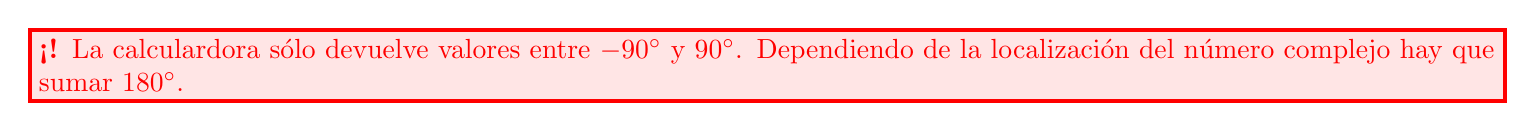
\begin{tikzpicture}
	\node[red, rectangle, draw, line width=1.5pt, text width=18.5cm, fill=red!10] {\textbf{¡!} La calculardora sólo devuelve valores entre $-90^\circ$ y $90^\circ$. Dependiendo de la localización del número complejo hay que sumar $180^\circ$.};
\end{tikzpicture}

\begin{center}
	\begin{tikzpicture}[scale=0.7]
		\draw[-latex] (-3, 0) -- (3,0);
		\draw[-latex] ( 0,-3) -- (0,3);
		\draw[lightblue] ( -2,2) -- (2,-2);
		\fill[lightblue] (-2,2) circle (2pt);
		\fill[lightblue] (2,-2) circle (2pt);
		\draw[blue] ( -2,-2) -- (2,2);
		\fill[blue] (-2,-2) circle (2pt);
		\fill[blue] (2,2) circle (2pt);
	\end{tikzpicture}
\end{center}

$\begin{array}{lcl}
	\text{Polar} & \longrightarrow & \text{Binómica}\\
	|z|_\theta &  \longrightarrow & z=|z|\cos\theta+\imath|z|\sin\theta
\end{array}$

\Ej

\begin{itemize}
	\item $1+\imath $
\end{itemize}
\begin{tikzpicture}[scale=0.5, baseline=(current bounding
	box.center)]
	\draw[-latex] (-3, 0) -- (3,0);
	\draw[-latex] ( 0,-3) -- (0,3);
	\draw[-latex, lightblue, line width=1.5pt] (0,0) -- (2,2)
	node[right] {$1+\imath $};
	\draw[dashed, lightblue, thick] (0,2) -- (2,2) -- (2,0);
\end{tikzpicture}
$\begin{array}{l}
	|1+\imath |=+\sqrt{1^2+1^2}=\sqrt{2}\\
	\theta=\arctan \frac{1}{1} =45^\circ=\frac{\pi}{4} \text{
		radianes} \\
	1+\imath =\sqrt{2}_{45^\circ}=\sqrt{2}e^{j\frac{\pi}{4}}
\end{array}$

\subsection{Representación matemática de una onda}
\begin{itemize}
	\item La función $\cos
	t=\frac{e^{jt}+e^{-\jmath  t}}{2},~t\equiv$tiempo.
\end{itemize}
\begin{tikzpicture}
	\draw[-latex] (-2,0)--(9,0);
	\draw[-latex] (0,-2)--(0,2);
	\draw[dashed] (-2,1)--(9,1);
	\draw[dashed] (-2,-1)--(9,-1);
	
	\draw[domain=2*pi:9, variable=\x, lightblue, dashed] plot
	({\x},{cos(\x r)});
	\draw[domain=-2:0, variable=\x, lightblue, dashed] plot
	({\x},{cos(\x r)});
	\draw[domain=0:2*pi, variable=\x, lightblue] plot ({\x},{cos(\x
		r)});
	\foreach \y in {-1, 1}
	\draw (0.1, \y) -- (-0.1, \y) node[left] {$\y$};
	\draw[lightblue] (pi/2, 0.1) -- (pi/2,-0.1) node[below]
	{$\pi\over2$};
	\draw[lightblue] (pi, 0.1) -- (pi,-0.1) node[below] {$\pi$};\draw[lightblue] (3*pi/2, 0.1) -- (3*pi/2,-0.1) node[below]
	{$3\pi\over2$};
	\draw[lightblue] (2*pi, 0.1) -- (2*pi,-0.1) node[below]
	{$2\pi$};
	\node[draw=black, rectangle, line width=1pt] at (12, 0)
	{Periodo\hspace{0.3cm}$T=2\pi$};
\end{tikzpicture}
\begin{itemize}
	\item La función $A\cos t=\frac{Ae^{jt}+Ae^{-\jmath  t}}{2}$
\end{itemize}
\begin{tikzpicture}
	\draw[-latex] (-2,0)--(7,0) node[right] {$t$};
	\draw[-latex] (0,-2)--(0,2);
	\draw[dashed] (0,1)--(7,1);
	\draw[dashed] (0,-1)--(7,-1);
	
	\draw[domain=0:2*pi, variable=\x, lightblue] plot ({\x},{cos(\x
		r)});
	\draw[lightblue] (pi/2, 0.1) -- (pi/2,-0.1) node[below]
	{$\pi\over2$};
	\draw[lightblue] (pi, 0.1) -- (pi,-0.1) node[below] {$\pi$};\draw[lightblue] (3*pi/2, 0.1) -- (3*pi/2,-0.1) node[below]
	{$3\pi\over2$};
	\draw[lightblue] (2*pi, 0.1) -- (2*pi,-0.1) node[below]
	{$2\pi$};
	\draw (0.1, 1) -- (-0.1, 1) node[left] {$A$};
	\draw (0.1, -1) -- (-0.1, -1) node[left] {$-A$};
	\node[draw=black, rectangle, line width=1pt] at (12, 0)
	{$A\equiv$ Amplitud de la onda};
\end{tikzpicture}

\begin{itemize}
	\item La función $\cos(wt)=\frac{e^{jwt}+e^{-\jmath wt}}{2}$
\end{itemize}
$wt=2\pi\longrightarrow t=\dfrac{2\pi}{w}=t$ período

Si $w$ es pequeño$\longrightarrow ~T$ es grande (pocas
oscilaciones)

\begin{tikzpicture}
	\draw[-latex] (-2,0)--(7,0) node[right] {$t$};
	\draw[-latex] (0,-2)--(0,2);
	
	\draw[domain=0:2*pi, variable=\x, lightblue] plot ({\x},{cos(\x
		r)});
	
	\foreach \y in {-1, 1}
	\draw (0.1, \y) -- (-0.1, \y) node[left] {$\y$};
	\draw[lightblue] (2*pi, 0.1) -- (2*pi,-0.1) node[below] {$T$};\end{tikzpicture}

Si $w$ es grande$\longrightarrow ~T$ es pequeño (muchas
oscilaciones)

\begin{tikzpicture}
	\draw[-latex] (-2,0)--(7,0) node[right] {$t$};
	\draw[-latex] (0,-2)--(0,2);
	
	\draw[domain=0:pi, variable=\x, lightblue] plot ({\x},{cos(2*\x
		r)});
	\draw[domain=pi:2*pi, variable=\x, lightblue, dashed] plot
	({\x},{cos(2*\x r)});
	
	\foreach \y in {-1, 1}
	\draw (0.1, \y) -- (-0.1, \y) node[left] {$\y$};
	\draw[lightblue] (pi, 0.1) -- (pi,-0.1) node[below] {$T$};
\end{tikzpicture}

Las ondas también se suelen manipular usando números complejos a partir de las identidades.

\[ \begin{array}{l}
	e^{\jm t}=\cos t+\jm \sin t\\
	e^{-\jm t}=\cos(-t)+\jm\sin(-t)=\left\{\begin{array}{l}
		\cos x \text{ es par}\\
		\sin x\text{ es impar}
	\end{array}\right\}=+\cos t-\jm\sin t
\end{array} \]

Sumando: $2\cos t=e^{\jm t}+e^{-\jm t}\longrightarrow\cos t=\dfrac{e^{\jm t+e^{-\jm t}}}{2}$

Restando: $e^{\jm t}-e^{-\jm t}=2\jm\sin t\longrightarrow\sin t=\dfrac{e^{\jm t-e^{-\jm t}}}{2\jm}$

Por tanto: \[\mathrm{Onda}=f(t)=A\cos(wt-\varphi)=\dfrac{A\cdot\left(e^{\jmath(wt-\varphi)}+e^{-\jmath (wt-\varphi)}\right)}{2}\]

\subsection{Raíces $n$-ésimas y raíces de polinomios}
\begin{wrapfigure}[3]{r}{0.3\textwidth}
	\begin{tikzpicture}[baseline=(current bounding box.center)]
		\draw (7.5,0) -- (12.5,0);
		\draw (10,-2.5) -- (10,2.5);
		\draw[lightblue] (10,0) circle (2);
		\fill[blue] (10,2) circle (3pt) node[above] {$~~~~z_1$};
		\fill[blue] (10,-2) circle (3pt) node[below] {$~~~~z_2$};
	\end{tikzpicture}
\end{wrapfigure}
Consideremos la ecuación $x^2+1=0$.

Buscamos $z\in\mathbb{C},~z=|z|e^{\im\theta}$ tal que $z^2+1=0$; $z^2=|z|^2e^{2\imath\theta}=-1=e^{\imath\pi}$ 

$\left\lbrace\begin{array}{l}
	|z|^2=1 \\
	2\theta=\pi+2k\pi
\end{array}\right.\longrightarrow\begin{array}{l}
	|z|=+\sqrt{1}=1 \\
	\theta=\dfrac{\pi}{2}+k\pi,~k=0,1,\dots
\end{array}$

$\begin{array}{l}
	k=0\longrightarrow\theta_1=\dfrac{\pi}{2}\\ k=1\longrightarrow\theta_2=\dfrac{\pi}{2}+\pi=\dfrac{3\pi}{2}\\
	k=2\longrightarrow\theta_3=\dfrac{\pi}{2}+2\pi=\dfrac{5\pi}{2}
\end{array}$